% Chapter Template

\chapter{Building a quantum processor} % Main chapter title

\label{Chapter4}

\noindent\hrulefill
\vspace{0.5cm} %\hspace{2cm}
%\small
\begin{flushright}
        ``\emph{Think big. Think fast. Think ahead. Ideas are no ones monopoly.}"
\\ 
--Dhirubhai Ambani \\
\end{flushright}

\vspace{0.5cm}


\noindent\hrulefill
\vspace{0.5cm} %\hspace{2cm}
\\
%\small
\hangindent=4cm
%\noindent
\\
The ultimate price in the high stakes game that is quantum computing these days, is a fault-tolerant large scale quantum computer, that is capable of solving relevant problems. In this chapter we are presenting our bet at it, employing the revelations of the flip-flop and nuclear qubit. We present ideas from an immediately achievable small quantum processor to a large scale architecture. 
\\ \\
\scriptsize
\hangindent=4cm
Parts of the work presented in this chapter have been published in:\\
G. Tosi, F. A. Mohiyaddin, V. Schmitt, \textbf{S. Tenberg}, R. Rahman,
G. Klimeck, A. Morello. ``Silicon quantum processor with robust long-distance qubit couplings.'' \textit{Nature communications} vol. 8, 450 (2017).\\
G. Tosi, F. A. Mohiyaddin, \textbf{S. Tenberg}, A. Laucht, A. Morello. ``Robust electric dipole transition at microwave frequencies for nuclear spin qubits in silicon.'' \textit{Physical Review B} vol. 98, 075313 (2018).\\
\\
\footnotesize
\hangindent=4cm
\textbf{The author acknowledges G. Tosi for the conception of the idea and J. O'Gorman for assistance with fault-tolerant quantum computation considerations. }\\

%\vspace{0.5cm}

\noindent \hrulefill
\clearpage

\normalsize

The flip-flop and the nuclear qubit, presented in chapters \ref{Chapter2} and \ref{Chapter3}, are excellent building blocks for a large scale quantum processor due to their long range couplings and low error rates. In this chapter ideas who incorporate them in a large quantum computing architecture are presented.   

\section{Quantum processor architectures}

\begin{figure}
	\centering
	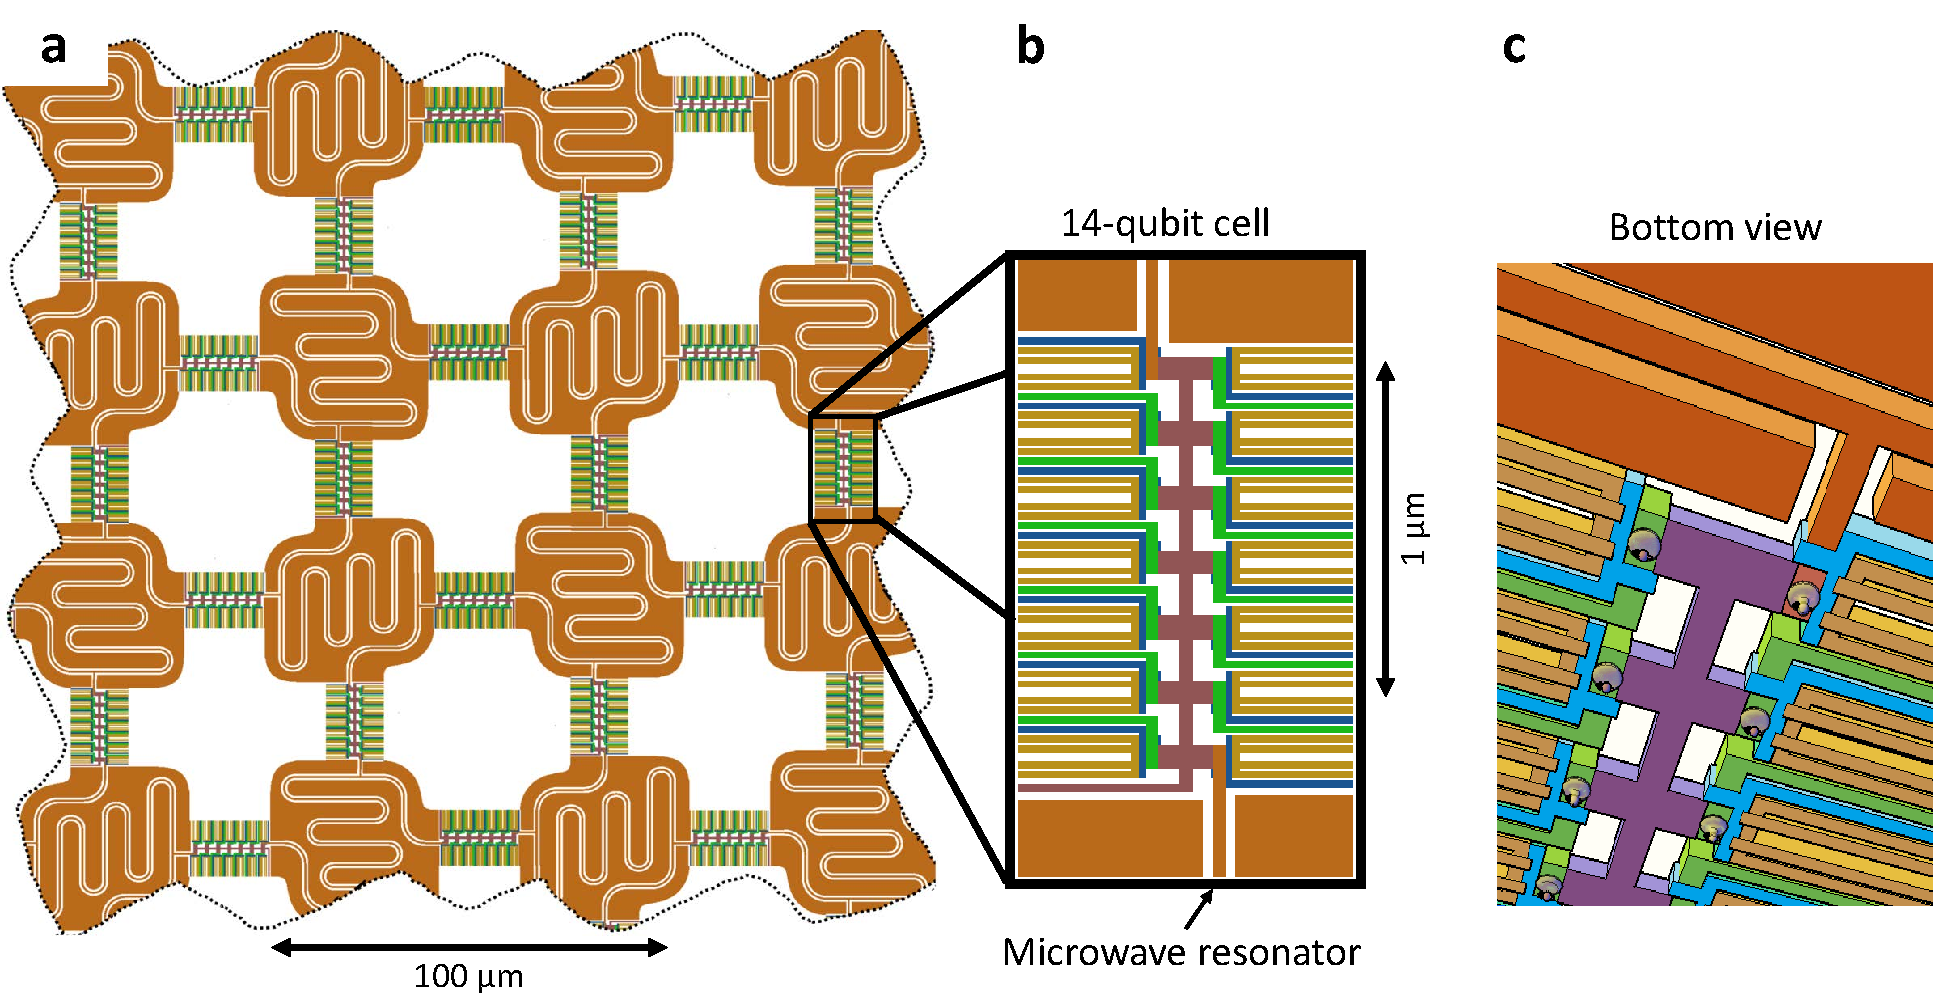
\includegraphics[width=\textwidth]{polished/qp_resonator.pdf}
	\caption[Hybrid quantum processor compatible with current university fabrication standards]{\textbf{Hybrid quantum processor compatible with current university fabrication standards}. Schematic view of a semi-large scale quantum processor which is feasible to build with current fabrication standards in our laboratory. \textbf{a} shows the processor where multiple 14-qubit cells are connected by superconducting resonators to a large computer. \textbf{b} shows the 14-qubit cell in detail from the top while \textbf{c} shows a bottom view. 14 flip-flop qubits are connected via nearest-neighbour or next-nearest-neighbour dipole-dipole interaction. Electrons can be loaded via a central reservoir (purple) and each qubit is read-out via a SET (yellow). The outer-most qubit is coupled to the resonator vacuum field with then allows for coupling to the next 14-qubit cell. }
	\label{fig:qp_14cell}
\end{figure}

Figure \ref{fig:qp_14cell} shows a simple version of a semi-large scale hybrid quantum computer, that only uses current standard 2D university fabrication techniques (see chapter \ref{sec:fabrication}) and could be thus fabricated in our laboratory. It consists out of 14-qubit cells connected by superconducting resonators. While the advantage of this processor is clearly its simplicity, the disadvantage is that parallel operations are very limited and thus quantum error correction cannot be applied as its overhead is too large. However, this processor could be used for small scale proof-of-principle experiments, like running algorithms such as Shor or Joszca-Deutsch \cite{Shor, Joszca}. 

\begin{figure}
	\centering
	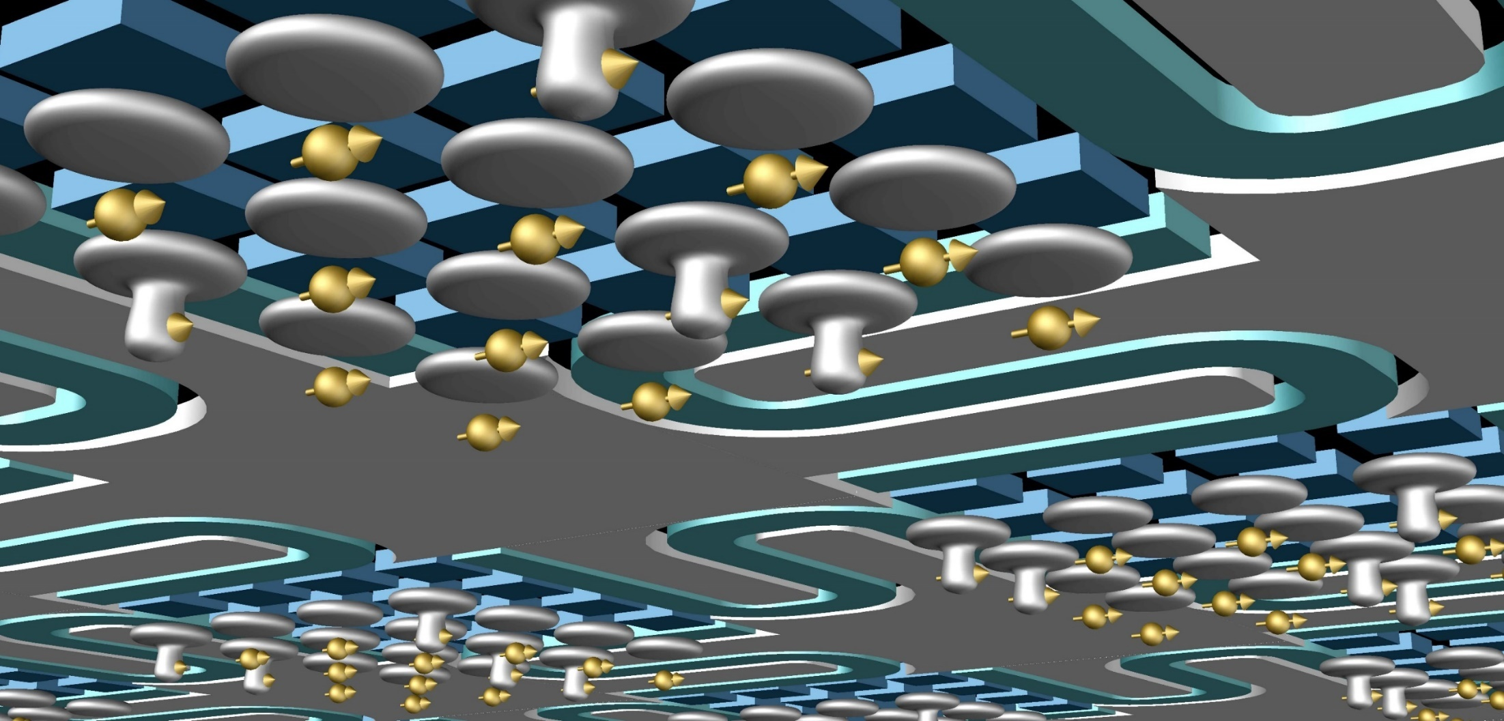
\includegraphics[width=\textwidth]{polished/qp_mixed.png}
	\caption[Large-scale hybrid quantum processor]{\textbf{Large-scale hybrid quantum processor}.
		\textbf{a} Schematic view of a large-scale quantum processor where 2D arrays of 16 dipolar coupled flip-flop qubits are connected via superconducting resonators. The drawing is not to scale; control lines and readout devices are not shown.}
	\label{fig:qp_mixed}
\end{figure}

Figure \ref{fig:qp_mixed} shows a large-scale quantum processor that consists out of 2D arrays of dipolar coupled flip-flop qubits, connected with superconducting resonators. Here, the size of the 2D flip-flop arrays is limited by the space required by read-out and control lines. In this case advanced error-correction codes may be implemented\cite{Knill2005,Nickerson2013,Terhal2015,Li2018a}, but the overhead it still large due to limited parallelism. This type of 2D arrays required 3D CMOS fabrication as the control and read-out lines need to be connected from above or below. 

Ultimately, one wants to build a full 2D array of only flip-flop qubits as presented in figure \ref{fig:qp_surfaceCode} for complete connectability and enhanced parallelism. This architecture allows proper quantum error correction as it is compatible with the surface code\cite{Fowler2012}: Each qubit is surrounded by ancilla qubits to detect errors. The qubits and ancillas interact with their neighbourings via the dipole-dipole interaction and all mutual qubit couplings are tunable and gateable. 

\begin{figure}
	\centering
	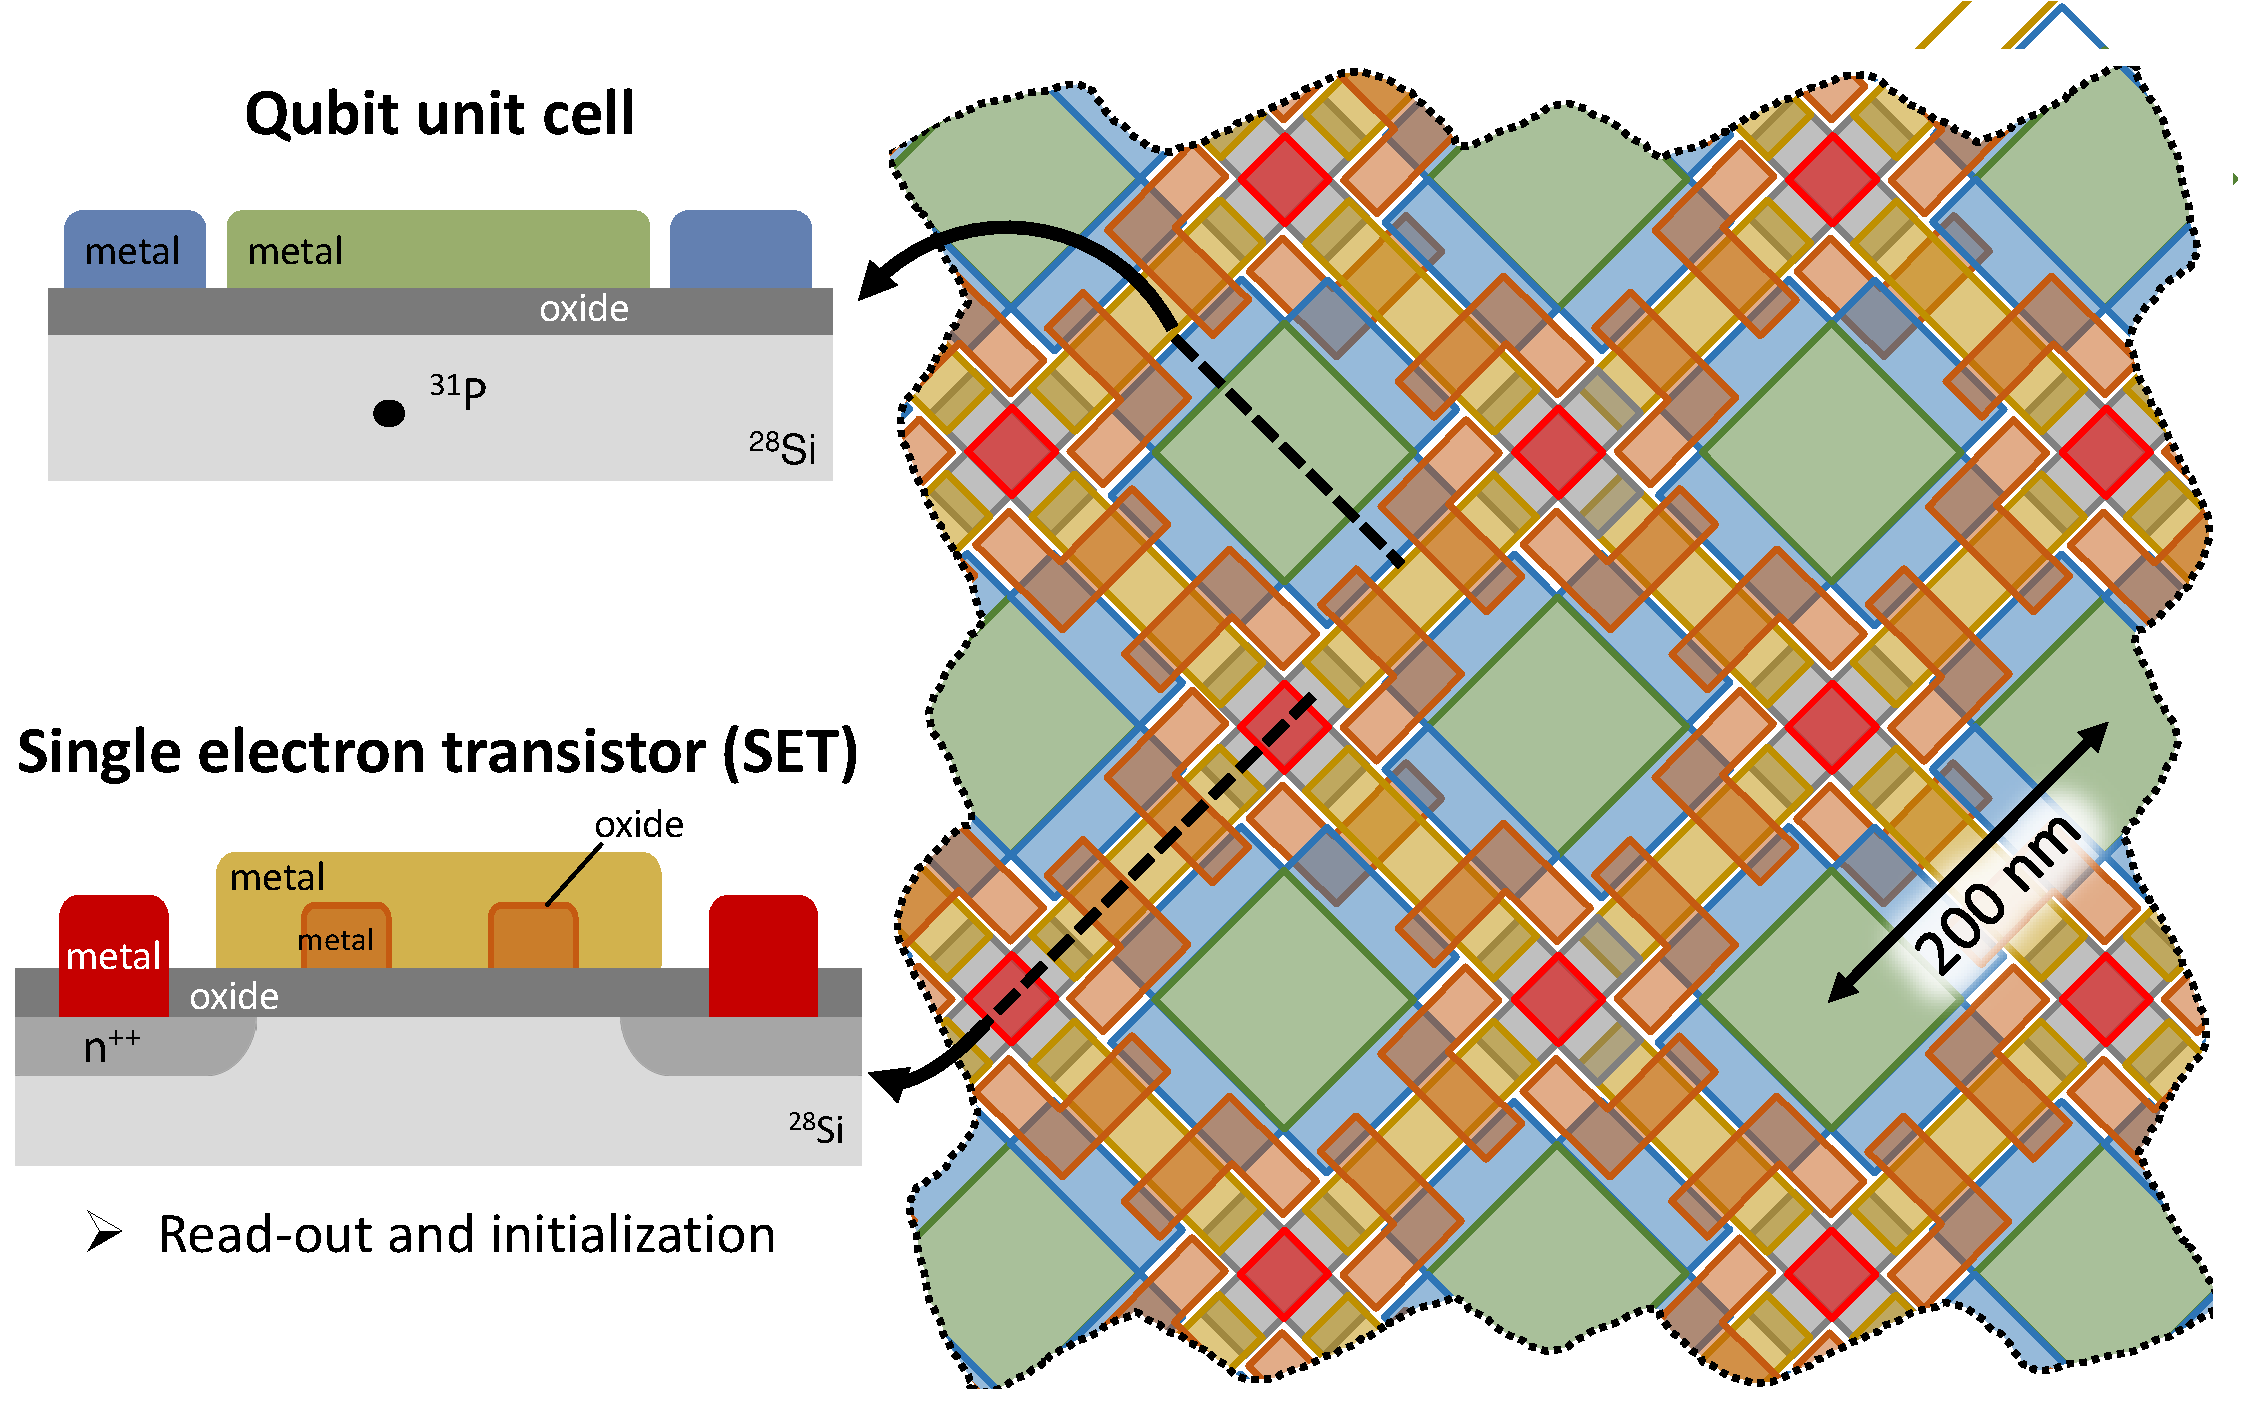
\includegraphics[width=\textwidth]{polished/surfaceCode.pdf}
	\caption[Surface code architecture]{\textbf{Surface code architecture}. Schematic view of a large-scale quantum processor that is compatible with the surface code \cite{Fowler2012}. Qubit unit cells consisting out of donors with a gate stack for tunnel coupling control are coupled via the dipole-dipole interaction. Every other qubit is used as an ancilla. Readout and initialization is performed via a SET. }
	\label{fig:qp_surfaceCode}
\end{figure}



\section{Operation principles of an electrically controlled donor quantum processor}

The fundamental operation principle for our donor quantum processor remains the same for the three suggested implementations. 

For initialization we use the n++ region and either the SET gate stack in Coulomb blockade or a designated reservoir to load an electron onto the donor. 
Idle qubits have electrons either at the interface or the donor, leaving them completely uncoupled to other qubits. Electrons are then adiabatically shifted towards the donor ionization point for quantum operations (see chapter \ref{sec:adiabatic_pc} and \ref{sec:elecDrive}).
Qubit read-out can be obtained by spin-dependent tunnelling into a cold charge reservoir, detected by a single-electron transistor \cite{Morello2010}. Read-out times can be $\sim1~\mu$s with cryogenic amplifiers \cite{Curry2015}, which is comparable to the time necessary to perform, for example, $\sim 20$ individual gates lasting $\sim 50$~ns each, in a surface code error correction protocol \cite{Fowler2012}.

\section{Nuclear qubit based processor}

Instead of flip-flop qubits, nuclear qubits can be used in the quantum processor. These have the advantage of having record coherence times $T_2 \gtrsim 30$~s (ref. \cite{Muhonen2014}) when the donor is ionization (the electron is at the interface). The magnetic drive can be a global, always-on field, e.g. supplied by a 3D microwave cavity. Quantum information can be swapped between the nuclear and the flip-flop qubit by simply applying an ESR $\pi$-pulse that excites the $\lvert{\downarrow\Downarrow}\rangle$ state to $\lvert{\uparrow\Downarrow}\rangle$ (Fig.~\ref{fig:hfchange}).
